%%% Notes on nitrogen CCSN and AGB star yields of N %%% 

\providecommand{\main}{..} 
\documentclass[\main/notes.tex]{subfiles} 

\begin{document} 
\begin{center} 
\textbf{{\Large CCSN and AGB Star Yields of Nitrogen}} 
\end{center} 

\noindent 
{\Large \textit{Core-Collapse Supernova Yields}} 
\par\noindent 
Empirically, nitrogen-to-oxygen ratios exhibit a plateau at 
$\log$(N/O)~$\approx$~-1.5 for~$\log$(O/H)~$\lesssim$~8 (see Fig. 1 of 
\citealp{Vincenzo2016} comparing~\citealp{Berg2012},~\citealp*{Izotov2012}, and 
\citealp{James2015} measurements). 
\twolineskip 
\textbf{What is the implied relation between the IMF integrated CCSN yields of 
nitrogen and oxygen?} 
\par\noindent 
The ratio of their yields can be related to the number densities of the two 
nuclei in the supernova ejecta via: 
\begin{equation} 
\ddfrac{y_\text{N}^\text{CC}}{y_\text{O}^\text{CC}} = 
\ddfrac{\mu_\text{N}n_\text{N}}{\mu_\text{O}n_\text{O}} 
\end{equation} 
where~$\mu_x$~is the mean molecular weight of a species~$x$~and~$n_x$ is the 
number of nuclei. Taking the ratio~$n_\text{N}/n_\text{O}$~from these observed 
results yields: 
\begin{equation} 
\ddfrac{y_\text{N}^\text{CC}}{y_\text{O}^\text{CC}} = 
\ddfrac{\mu_\text{N}}{\mu_\text{O}}10^{\log\text{(N/O)}} 
\end{equation} 
Though supernova ejecta may produce different isotopic ratios of N than AGB 
stars, potentially  
altering the ratio~$\mu_\text{N}/\mu_\text{O}$, taking~$\mu_\text{N}$ = 14.007 
and~$\mu_\text{O}$ = 15.999 from a periodic table suggests that, with the 
previously adopted~$y_\text{O}^\text{CC}$ = 0.015 (e.g.~\citealp*{Weinberg2017}; 
\citealp{Johnson2020,Johnson2021}), this suggests 
\begin{equation} 
y_\text{N}^\text{CC} = \ddfrac{\mu_\text{N}}{\mu_\text{O}}10^{\log\text{(N/O)}} 
y_\text{O}^\text{CC} = \ddfrac{14.007}{15.999}10^{-1.5}(0.015) \approx 
4.15\times10^{-4} 
\end{equation} 
\twolineskip 
\textbf{Can this be understood from theoretically predicted yields?} 

\begin{figure*}[!t] 
\centering 
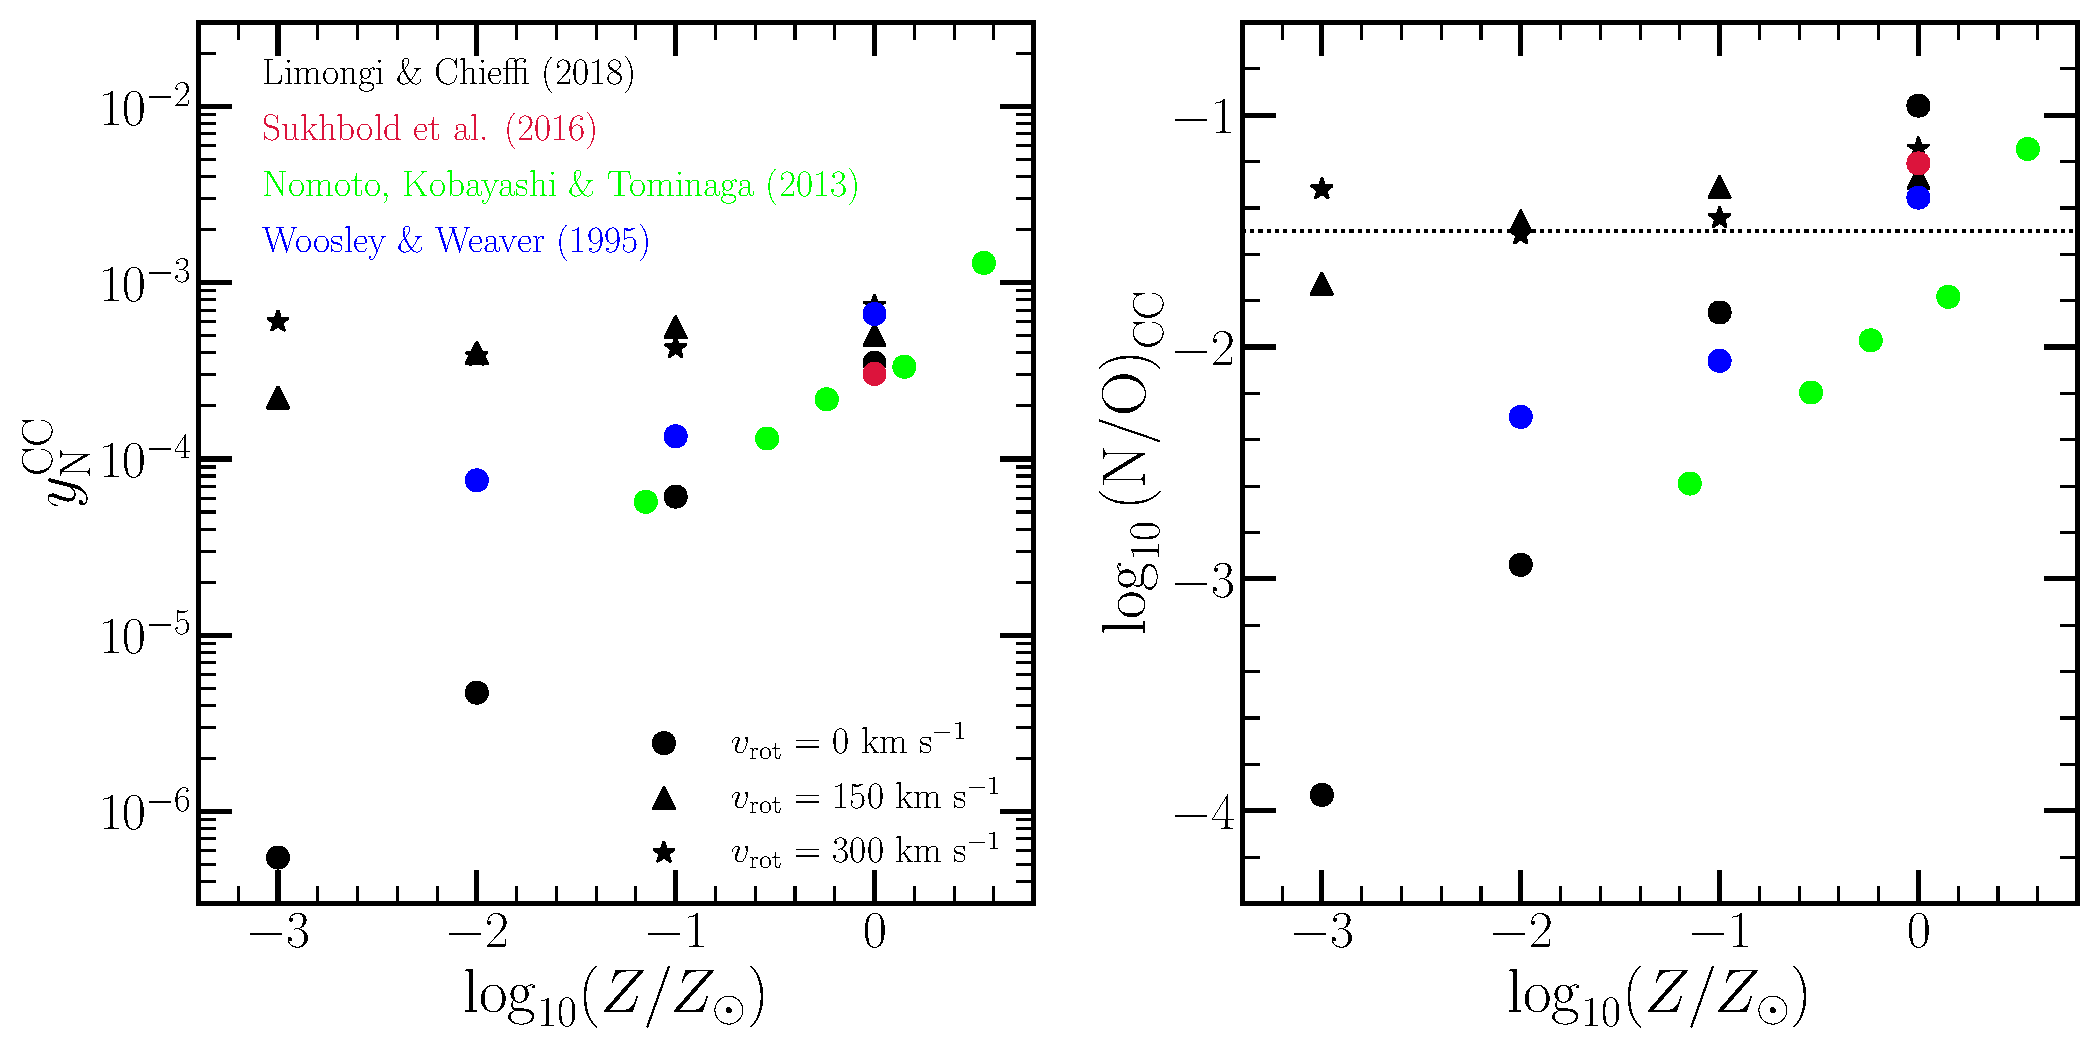
\includegraphics[scale = 0.45]{\main/yields/n_cc_yields.pdf} 
\caption{
\textbf{Right}: IMF-integrated CCSN yields of N computed with VICE using the 
\citet{Limongi2018} (black),~\citet{Sukhbold2016} (crimson),~\citet{Nomoto2013} 
(lime), and~\citet{Woosley1995} (blue) yield sets. 
\textbf{Left}: IMF-integrated nitrogen-to-oxygen yield ratios computed with 
VICE for the same studies. 
The~\citet{Limongi2018} yields are calculated with progenitor rotational 
velocities of~$v_\text{rot}$ = 0 (circles), 150 (triangles), and 300 km/s 
(stars). 
All other studies only report yields for non-rotating progenitors. } 
\label{fig:n_cc_yields} 
\end{figure*} 

\noindent 
The left panel of Figure~\ref{fig:n_cc_yields} presents the IMF-integrated 
yields~$y_\text{N}^\text{CC}$~computing with VICE using the~\citet{Limongi2018}, 
\citet{Sukhbold2016},~\citet{Nomoto2013}, and~\citet{Woosley1995} CCSN yield 
tables, with~\citet{Limongi2018} being the only study which reports yields for 
rotating progenitors. 
Broadly, the non-rotating predictions are consistent with one another, and 
predict a significant metallicity dependence; the lowest metallicity progenitor 
from~\citet{Woosley1995} predict somewhat higher yields overall, but this could 
have to do with this being the only yield set for which we can calculate 
only~\textit{gross} yields rather than~\textit{net} yields. 
The rotating progenitors from~\citet{Limongi2018}, however, predict that the 
yield should be considerably enhanced by rotation. 
They interpret this as being due to the interplay between the core helium and 
hydrogen burning shells triggered by rotation-induced instabilities, which 
drives the synthesis of all products of CNO, not just~$^{14}$N (see their 
abstract). 
These yields predict a relatively metallicity-independent~$y_\text{N}^\text{CC}$ 
of~$\sim5\times10^{-4}$, in surprisingly good agreement with the empirically 
derived value of~$4.15\times10^{-4}$. 
\par 
The right panel of Figure~\ref{fig:n_cc_yields} presents the IMF-integrated 
nitrogen-to-oxygen ratios predicted by the same studies for the same 
combinations of metallicity and rotational velocity. 
The flat, dotted black line denotes~$\log_{10}\text{(N/O)}_\text{CC}$ = -1.5, 
the value empirically derived from observations~\citep{Vincenzo2016, 
Berg2012, Izotov2012, James2015}. 
The rotating progenitor models from~\citet{Limongi2018} do the best job of 
reproducing this ratio in theoretical models of core collapse supernova ejecta; 
the other models do not include rotation, which appears to play a key role in 
establishing this empirical result. 

% \newpage\noindent 
\twolineskip 
\textbf{What is the implied plateau in [N/O]?} 
\par\noindent 
[N/O] and~$\log$(N/O) are directly related, but one is relative to the sun 
while the other is just a ratio of number densities. Expanding [N/O]: 
\begin{subequations}\begin{align} 
\text{[N/O]} &= \text{[N/H]} - \text{[O/H]} \\ 
&= \log_{10}\left(\ddfrac{Z_\text{N}}{Z_{\text{N},\odot}}\right) - 
\log_{10}\left(\ddfrac{Z_\text{O}}{Z_{\text{O},\odot}}\right) 
\\ 
&= \log_{10}\left(\ddfrac{Z_\text{N}}{Z_\text{O}}\right) - \log_{10}\left(
\ddfrac{Z_{\text{N},\odot}}{Z_{\text{O},\odot}}\right) 
\end{align}\end{subequations} 
Zooming in on the~$Z_\text{N}/Z_\text{O}$ term: 
\begin{subequations}\begin{align} 
\log_{10}\left(\ddfrac{Z_\text{N}}{Z_\text{O}}\right) &= 
\log_{10}\left(\ddfrac{\mu_\text{N}n_\text{N}}{\mu_\text{O}n_\text{O}}\right) \\ 
&= \log_{10}\left(\ddfrac{\mu_\text{N}}{\mu_\text{O}}\right) + \log_{10}\left(
\ddfrac{n_\text{N}}{n_\text{O}}\right) 
\end{align}\end{subequations} 
where~$\mu$~and~$n$~are again the mean molecular weight and number of some 
species~$x$. The term~$\log_{10}\left(n_\text{N}/n_\text{O}\right)$~is exactly 
the~$\log$(N/O) value which~\citet{Berg2012},~\citet*{Izotov2012}, and 
\citet{James2015} measured to be~$\sim$-1.5. Plugging this in: 
\begin{subequations}\begin{align} 
\text{[N/O]} &= \log_{10}\left(\ddfrac{\mu_\text{N}}{\mu_\text{O}}\right) + 
\log_{10}\left(\ddfrac{n_\text{N}}{n_\text{O}}\right) - \log_{10}\left(
\ddfrac{Z_{\text{N},\odot}}{Z_{\text{O},\odot}}\right) 
\end{align}\end{subequations} 
Taking~$\mu_\text{N}$~= 14.007 and~$\mu_\text{O}$~= 15.999 again, with the 
empirical result of~$\log_{10}\left(n_\text{N}/n_\text{O}\right)$~= -1.5 and 
the~\citet{Asplund2009} solar photospheric composition of~$Z_{\text{N},\odot}$ 
= $6.91\times10^{-4}$~and~$Z_{\text{O},\odot}$~= 0.00572, yields the following: 
\begin{equation} 
\text{[N/O]}_\text{plateau} = -0.64 
\end{equation} 

\twolineskip 
{\Large \textit{Asymptotic Giant Branch Star Yields}} 
\par\noindent 

\begin{figure*}
\centering 
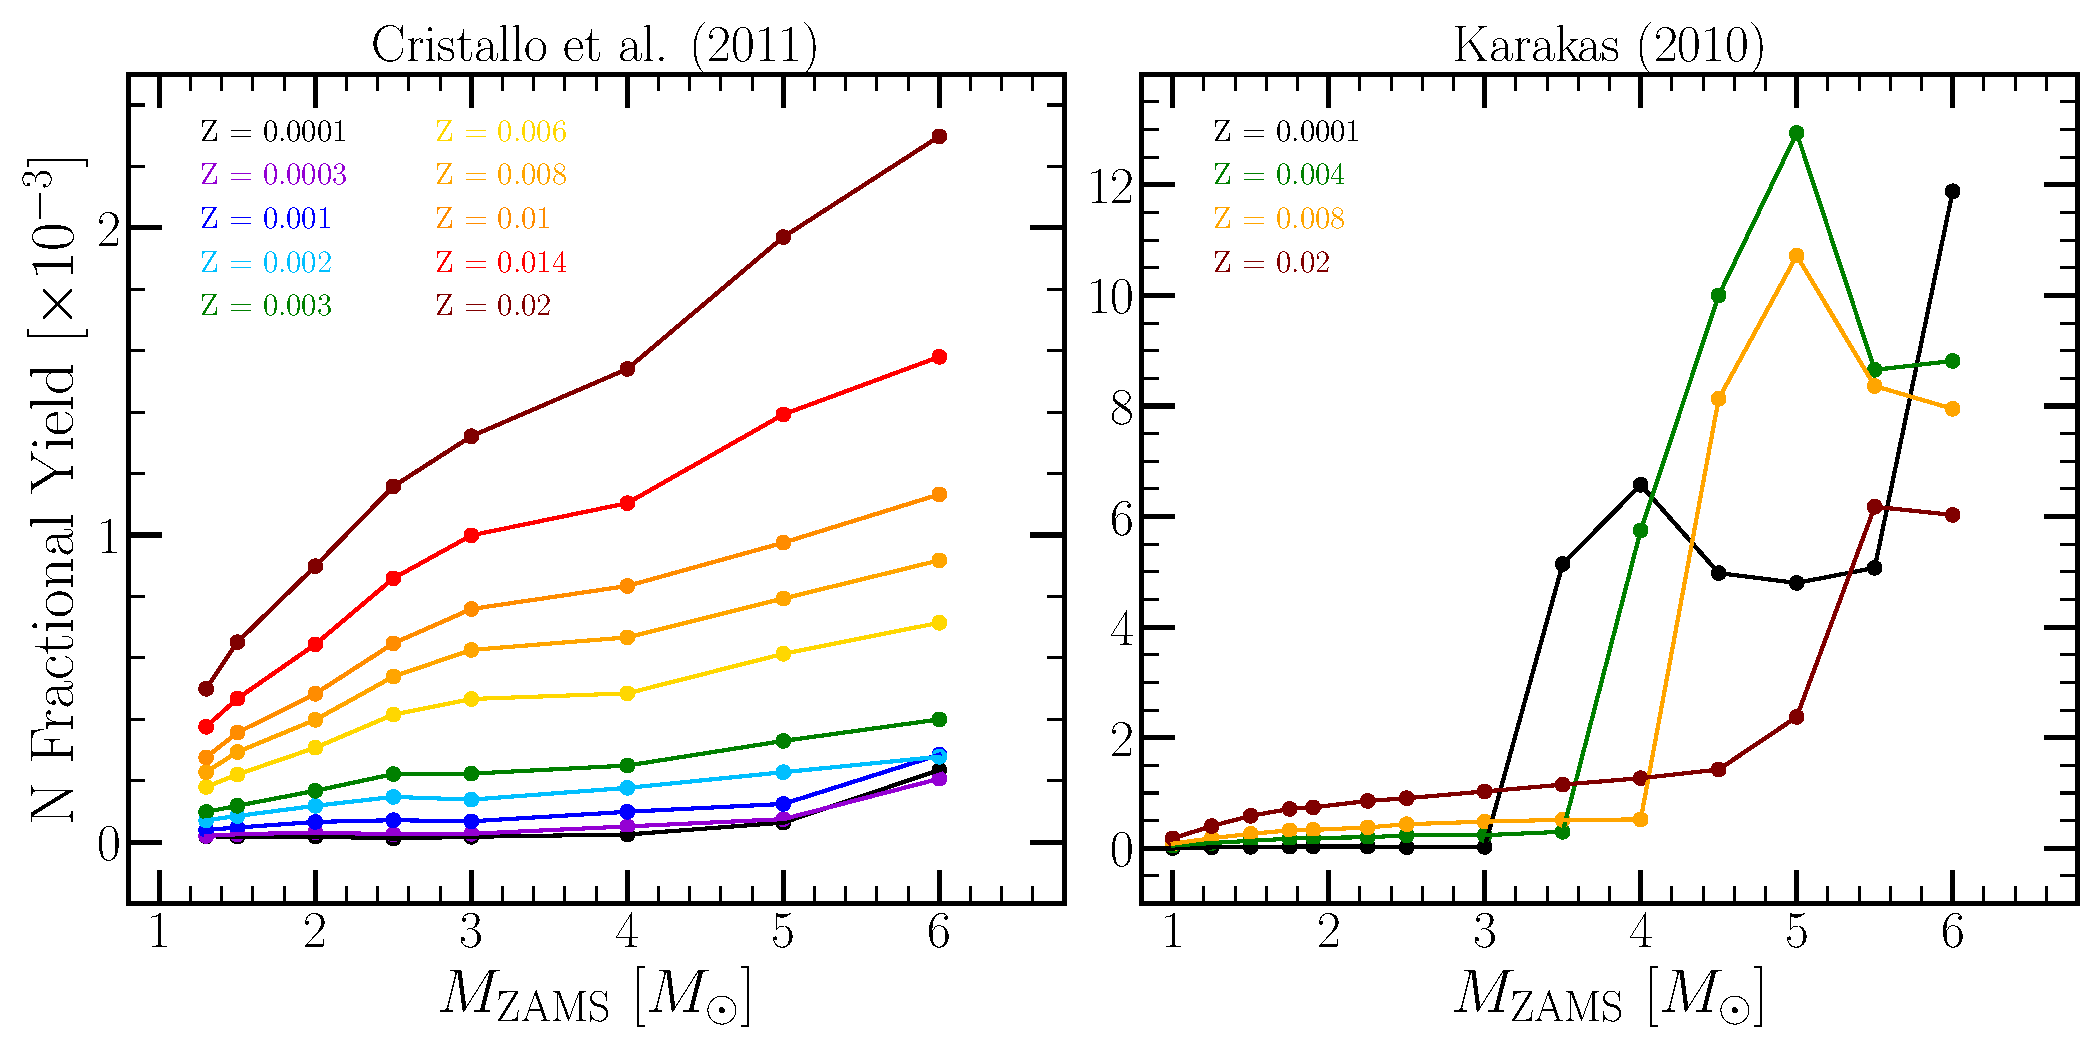
\includegraphics[scale = 0.45]{\main/yields/n_agb_yields.pdf} 
\caption{Fractional yields of N as a function of progenitor zero age main 
sequence mass at the metallicities at which~\citet{Cristallo2011} (left) and 
\citet{Karakas2010} report yields.} 
\label{fig:n_agb_yields} 
\end{figure*} 

\begin{figure*} 
\centering 
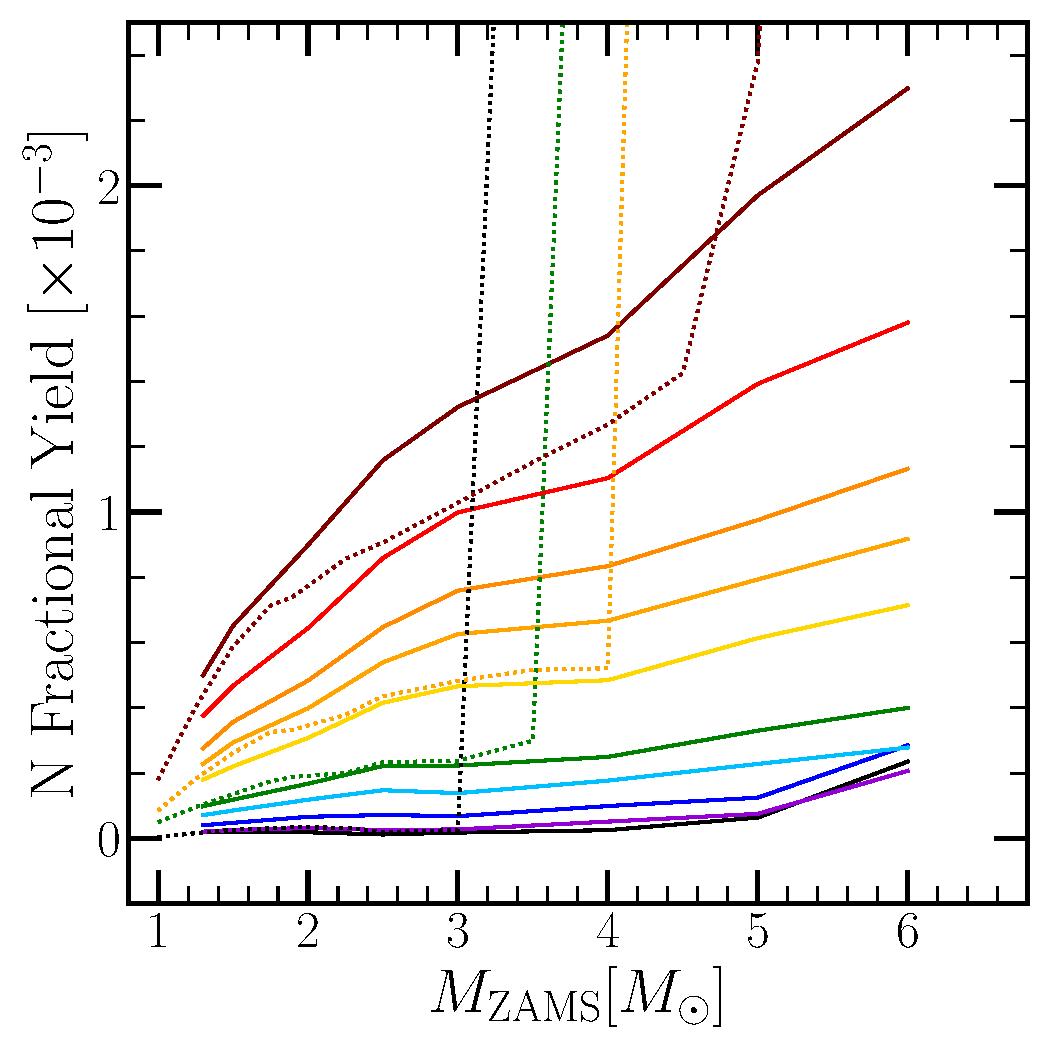
\includegraphics[scale = 0.5]{\main/yields/n_agb_yields_comp.pdf} 
\caption{The same as figure~\ref{fig:n_agb_yields}, but with the 
\citet{Cristallo2011} (solid) and~\citet{Karakas2010} yields plotted on the 
same set of axes for comparison. } 
\label{fig:n_agb_yields_comp} 
\end{figure*} 

Figure~\ref{fig:n_agb_yields} presents the fractional yields of N as a function 
of progenitor zero age main sequence (ZAMS) mass and metallicity as reported in 
the FRUITY database~\citep{Cristallo2011} and by~\citet{Karakas2010}. Both 
models show the metallicity-dependent nature of seconday nitrogen production, 
whose fractional yields increase with progenitor mass at fixed metallicity. 
Secondary nitrogen production refers to the production of~$^{14}$N at the 
expense of C and O in the CNO cycle; the nuclear reaction network of the CNO 
cycle: 

\twolineskip 
$^{12}$C(p,$\gamma$)$^{13}$N(,$\beta^+$)$^{13}$C(p,$\gamma$)$^{14}$N(p,$\gamma$)
$^{15}$O(,$\beta^+$)$^{15}$N(p,$\alpha$)$^{12}$C 

\twolineskip 
In this chain, the~$^{14}$N(p,$\gamma$)$^{15}$O reaction is particularly slow, 
and for this reason, the net effect of the CNO cycle is to turn all of the C 
and O into~$^{14}$N at their expense. 
\par 
By omparing the left- and right-hand panels of Fig.~\ref{fig:n_agb_yields}, 
it's clear that the~\citet{Karakas2010} predicts secondary nitrogen production 
to be a much stronger effect than~\citet{Cristallo2011}; the yields from high 
mass stars are over an order magnitude larger in~\citet{Karakas2010} than in 
\citet{Cristallo2011} at all reported metallicities except solar. 
\citet{Karakas2010} also predicts a much more complicated mass-dependence than 
does~\citet{Cristallo2011}. {\color{red} Intuitively, I would think that 
secondary N yields should be nothing but monotonic with metallicity. Rotation 
may induce some interesting effects, but unfortunately the~\citet{Karakas2010} 
paper makes no mention of rotation. They were primarily interested in the 
effect of updates to the~$^{13}$C($\alpha$,n)$^{16}$O reaction on light-element 
nucleosynthesis. I'm assuming this means they were using non-rotating models, 
but if this ends up being discussed in a paper I should email Amanda Karakas 
to verify. } 
\par 
\textbf{How consistent are the two studies up to~$\sim$3-4~\msun?} 
Figure~\ref{fig:n_agb_yields_comp} compares the two sets of yields on the same 
plot, with the~\citet{Cristallo2011} set shown in solid lines and the 
\citet{Karakas2010} set in dotted lines. 
The two are broadly consistent with one another up this threshold mass, at 
which point the secondary nitrogen yields as reported by~\citet{Karakas2010} 
become considerably large in comparison. 






%%% Analytic notes on equilibrium abundance of nitrogen %%% 

\twolineskip 
\null 
\twolineskip 
{\Large \textit{Analytic Motivation of Nitrogen Yields}} 
\par\noindent 
Can we come up with a mathematical framework with which to relate a late-time 
[N/O]-[O/H] relation and nitrogen yields using equilibrium arguments in simple 
one-zone models? 
\par 
\textbf{The time-derivative of the main sequence mass fraction} 
\par\noindent 
The main sequence mass fraction is the fraction of a stellar population's mass 
still on the main sequence. 
If the post-main sequence lifetime is approximated to be zero, this is also the 
star cluster mass fraction. 
It is given by: 
\begin{equation} 
h = \ddfrac{
	\int_l^{\mto} m\frac{dN}{dm} dm  
}{
	\int_l^u m\frac{dN}{dm} dm 
} , 
\end{equation}
where~$l$ and~$u$ are the lower and upper mass limits on star formation, 
respectively,~$dN/dm$ is the adopted stellar IMF, and~\mto~is the turnoff mass 
in solar masses. 
Allowing the constant~$\xi$ to represent the normalization of the IMF, zooming 
in on the denominator: 
\begin{subequations}\begin{align} 
\int_l^u &= \xi m^{1 - \alpha} dm \\ 
&= \frac{\xi}{2 - \alpha} m^{2 - \alpha}\Big|_l^u \\ 
&= \frac{\xi}{0.7}m^{0.7}\Big|_{0.08}^{0.5} - 
\frac{\xi}{0.6}m^{-0.3}\Big|_{0.5}^{100} \\ 
&= 2.239\xi 
\end{align}\end{subequations} 
where the power-law indeces and constants are appropriate for 
a~\citet{Kroupa2001} IMF (with 0.6 in the second denominator rather than 0.3 
to account for piece-wise continuity) assuming~$l$ = 0.08 and~$u$ = 100. 
In the numerator of~$h$, only the quantity~\mto~varies with time. 
The time-derivative then follows trivially from the stellar IMF. 
\begin{subequations}\begin{align} 
\dot{h} &= \frac{1}{2.239\xi} \frac{d}{dt} 
\int_l^{\mto} m \frac{dN}{dm} dm 
\\ 
&= \frac{1}{2.239\xi} \frac{d}{d\mto} 
\int_l^{\mto} m \frac{dN}{dm} dm \frac{d\mto}{dt} 
\\ 
&= \frac{\mto}{2.239\xi} \frac{dN}{dm} \Big|_{\mto} \frac{d\mto}{dt} 
\\ 
&= \frac{\mto}{2.239\xi} A\xi \mto^{-\alpha} \frac{d\mto}{dt} 
\end{align}\end{subequations} 
where~$\alpha$ = 1.3 (2.3) for~$0.08 \leq m \leq 0.5$ ($m \geq 0.5$) according 
to the~\citet{Kroupa2001} IMF and~$A$ = 1 (0.5) for the same mass ranges 
ensures piece-wise continuity of the IMF. 
However, since the lifetime of an~$m$ = 0.5 star is very long ($\sim$113 Gyr 
for~\vice's approximation),~$A$ = 0.5 and~$\alpha$ = 2.3 always for the sake of 
this calculation. 
\begin{subequations}\begin{align} 
&= \frac{0.5\mto}{2.239\xi} \xi\mto^{-2.3} \frac{d\mto}{dt} 
\\ 
&= 0.223\mto^{-1.3} \frac{d\mto}{dt} 
\label{eq:hdot:terms_of_mto} 
\end{align}\end{subequations} 
The turnoff mass at a given time, as approximated in~\vice, is given by 
\begin{equation} 
\mto = \left(\frac{t}{\tau_\odot}\right)^{-1/3.5} = 
\left(\frac{t}{\tau_\odot}\right)^{-2/7}, 
\label{eq:mto:def} 
\end{equation} 
where~$\tau_\odot$ is the main sequence lifetime of the sun. 
Differentiating with time: 
\begin{equation} 
\frac{d\mto}{dt} = \frac{-2}{7\tau_\odot} 
\left(\frac{t}{\tau_\odot}\right)^{-9/7} 
\label{eq:mto:time_derivative} 
\end{equation} 
Plugging equations~\ref{eq:mto:def} and~\ref{eq:mto:time_derivative} into 
equation~\ref{eq:hdot:terms_of_mto}: 
\begin{subequations}\begin{align} 
\dot{h} &= 0.223\left(\frac{t}{\tau_\odot}\right)^{2.6/7} 
\left(\frac{-2}{7\tau_\odot}\right)\left(\frac{t}{\tau_\odot}\right)^{-9/7} 
\\ 
&= \frac{-0.0637}{\tau_\odot}\left(\frac{t}{\tau_\odot}\right)^{-6.4/7} 
\\ 
&= \frac{-0.0637}{\tau_\odot}\left(\frac{t}{\tau_\odot}\right)^{-32/35} 
\label{eq:hdot} 
\end{align}\end{subequations} 

This form for~$\dot{h}$ is appropriate for the~\citet{Kroupa2001} IMF with a 
mass range of star formation defined by~$l$ = 0.08 and~$u$ = 100 assuming a 
mass-lifetime relationship given by~\ref{eq:mto:def}. 
However, the time-dependence is set not by the IMF but by the mass-lifetime 
relationship; the IMF affects only the normalization of~$\dot{h}$. 

\twolineskip 
\textbf{The Enrichment Rate from AGB Stars} 
\par\noindent 
Next, equation~\ref{eq:hdot} must be plugged into the equation describing the 
enrichment rate from AGB stars: 
\begin{equation} 
\dot{M}_\text{N}^\text{AGB} = -\int_0^T y_\text{N}^\text{AGB}(\mto(T - t), 
Z_\text{ISM}(t)) \dot{M}_\star(t) \dot{h}(T - t) dt 
\end{equation} 
In general, the SFR~$\dot{M}_\star$ can have any time-dependence, and the 
gas-phase abundance of the star forming reservoir~$Z_\text{ISM}$ as a function 
of time has some complicated form which depends on the SFH. 
As a first guess though, we can assume a constant SFR, and since nitrogen 
production is dominated by young stellar populations, most of the enrichment 
should be coming from stars near the equilibrium abundance. 
Furthermore, the AGB star yields of N appear to depend more or less linearly on 
initial stellar mass. 
As a first guess then, assume that~$y_\text{N}^\text{AGB} = \xi\mto Z$ 
where~$\xi$ is simply a normalizing constant. 
Under these assumptions this integral can be re-expressed as: 
\begin{subequations}\begin{align} 
\dot{M}_\text{N}^\text{AGB} &= -\int_0^T \xi\mto(T - t) Z_\text{eq} 
\dot{M}_\star \dot{h}(T - t) dt 
\\ 
&= \xi Z_\text{eq} \dot{M}_\star \int_0^T 
\left(\frac{T - t}{\tau_\odot}\right)^{-2/7} \frac{0.0637}{\tau_\odot} 
\left(\frac{T - t}{\tau_\odot}\right)^{-6.4/7} dt 
\\ 
&= \frac{0.0637\xi Z_\text{eq}\dot{M}_\star}{\tau_\odot} 
\int_0^T \left(\frac{T - t}{\tau_\odot}\right)^{-8.4/7} dt 
\\ 
&= \frac{0.0637\xi Z_\text{eq}\dot{M}_\star}{\tau_\odot} 
\left[\left(\frac{-7}{1.4}\right)\left(\frac{T - t}{\tau_\odot}\right)^{-1.4/7}
(-\tau_\odot) 
\right]_0^T 
\\ 
&= 0.3185\xi Z_\text{eq}\dot{M}_\star
\left[\left(\frac{\tau_8}{\tau_\odot}\right)^{-1.4/7} - 
\left(\frac{T}{\tau_\odot}\right)^{-1.4/7}\right] 
\\ 
&= 0.3185\xi Z_\text{eq}\dot{M}_\star \left[
\left(\frac{\tau_8}{\tau_\odot}\right)^{-1.4/7} - 
\left(\frac{T}{\tau_\odot}\right)^{-1.4/7}\right] 
\\ 
&= 1.064 \xi Z_\text{eq} \dot{M}_\star 
\end{align}\end{subequations} 
In the second to last equality, the upper bound of the integral is evaluated 
at~$T - \tau_8$ rather than inserting an infinity; mathematically, the infinite 
value reflects the divergence of~$\dot{h}$ for zero-age stellar populations. 
However, the integral really should only be evaluated up to the simulation time 
minus the lifetime of an 8~\msun~star ($\tau_8$), since these are the most 
massive AGB stars in these models. 
The final equality assumes a lifetime of~$\tau_\odot8^{-3.5}$ Gyr as the 
lifetime of an 8~\msun~star,~$T$ = 13.2 Gyr as the simulation time, 
and~$\tau_\odot$ = 10 Gyr as the lifetime of the sun. 
\par 
The rate of CCSN enrichment reflects the yield at the equilibrium metallicity: 
\begin{equation} 
\dot{M}_\text{N}^\text{CC} = y_\text{N}^\text{CC}(Z_\text{eq})\dot{M}_\star 
\end{equation} 
\twolineskip 
\textbf{The Equilibrium Abundance of Nitrogen} 
\par\noindent 
The equilibrium metallicity for a constant SFH then corresponds to solving 
for~$\dot{Z}_\text{N}$ = 0 from the following, derived from the enrichment 
equation and the equilibrium arguments from~\citet*{Weinberg2017}: 
\begin{equation} 
\dot{Z}_\text{N} = \frac{1}{\dot{M}_\star\tau_\star} 
\left[\dot{M}_\text{N}^\text{CC} + \dot{M}_\text{N}^\text{AGB} - Z_\text{N} 
\dot{M}_\star(1 + \eta - r)\right] 
\end{equation} 
When~$\dot{Z}_\text{N}$ = 0,~$Z_\text{N} = Z_\text{N,eq}$, the equilibrium 
abundance of nitrogen. It then follows: 
\begin{subequations}\begin{align} 
Z_\text{N,eq}\dot{M}_\star(1 + \eta - r) &= 
\dot{M}_\text{N}^\text{CC} + \dot{M}_\text{N}^\text{AGB} 
\\ 
&= y_\text{N}^\text{CC}(Z_\text{eq})\dot{M}_\star + 1.064\xi Z_\text{eq} 
\dot{M}_\star 
\\ 
Z_\text{N,eq} &= \frac{
	y_\text{N}^\text{CC}(Z_\text{eq}) + 1.064\xi Z_\text{eq} 
}{
	1 + \eta - r 
}
\end{align}\end{subequations} 
Since nitrogen has metallicity dependent yields,~$Z_\text{eq}$ is 
the~\textit{total} abundance. 
The constant~$\xi$ specifies the normalization of the nitrogen AGB star yield 
assuming a linear dependence on both turnoff mass and metallicity given 
by~$y_\text{N}^\text{AGB} = \xi\mto Z$. 
This form does make the assumption that all AGB star production is coming from 
younger stellar populations near the equilibrium abundance. 
Since N production timescales are quite short (~$\sim$100 Myr), this assumption 
is likely accurate enough. 
The constant~$\xi$ could be determined by a fit to the~\citet{Cristallo2011} or 
the~\citet{Ventura2013} models, also absorbing whatever prefactor is built in; 
the~\citet{Karakas2010} yields likely couldn't be used for this since they do 
not show a linear dependence of~$y_\text{N}^\text{AGB}$ on progenitor mass. 
\par 
The basic motivation of this is that at a given radius~\rgal, the equilibrium 
abundance of oxygen is known by the scaling of~$\eta$ to set the metallicity 
gradient. 
By assuming that the equilibrium abundance of nitrogen reflects the observed 
[N/O]-[O/H] relation, the only remaining unknowns in this formalism are the 
yields. 
This procedure can then be tested with~\vice's numerical simulations allowing 
migration, time-dependent SFHs, etc. to test how robust the predictions are to 
the assumptions built into this analytic argument. 




% \bibliographystyle{mnras}  
% \bibliography{\main/notes} 
\biblio 

\end{document} 

